\chapter{Dynamic Programming}
Transforming complex problems into a sequence of subproblems whose solutions can be used to construct a solution for the bigger and original problem.
It also is a general framework for analyzing and solving optimization problems effectively and fast\footnote{Usually optimization problems require exponential time to be solved.}.

Dynamic programming decompose large problem in a collection of small problems which can be solved in linear order (forming a implicit conceptual DAG) one after the other, from the \textit{smallest} to the \textit{largest} and using solution to the small ones to solve the bigger ones. 

\section{DAG shortest Path}
Probably one of the easiest example that can depict the concept behind DP is the problem of computing the shortest path in a DAG (because of the analogy with DP itself which linearize problems and the fact that DAGs can be linearized s.t. all the edges point forward).

\begin{framed}
A DAG is a graph such that exists a topological ordering (see figure \ref{fig:DAGsort}) of nodes $v1,v2, \ldots,v_n$ (we assign an differen interger to each  node) s.t. for each edge $(i,j)$ we have that $i<j$.
	
\end{framed}

	\begin{figure}
	\label{fig:DAGsort}
	\centering
	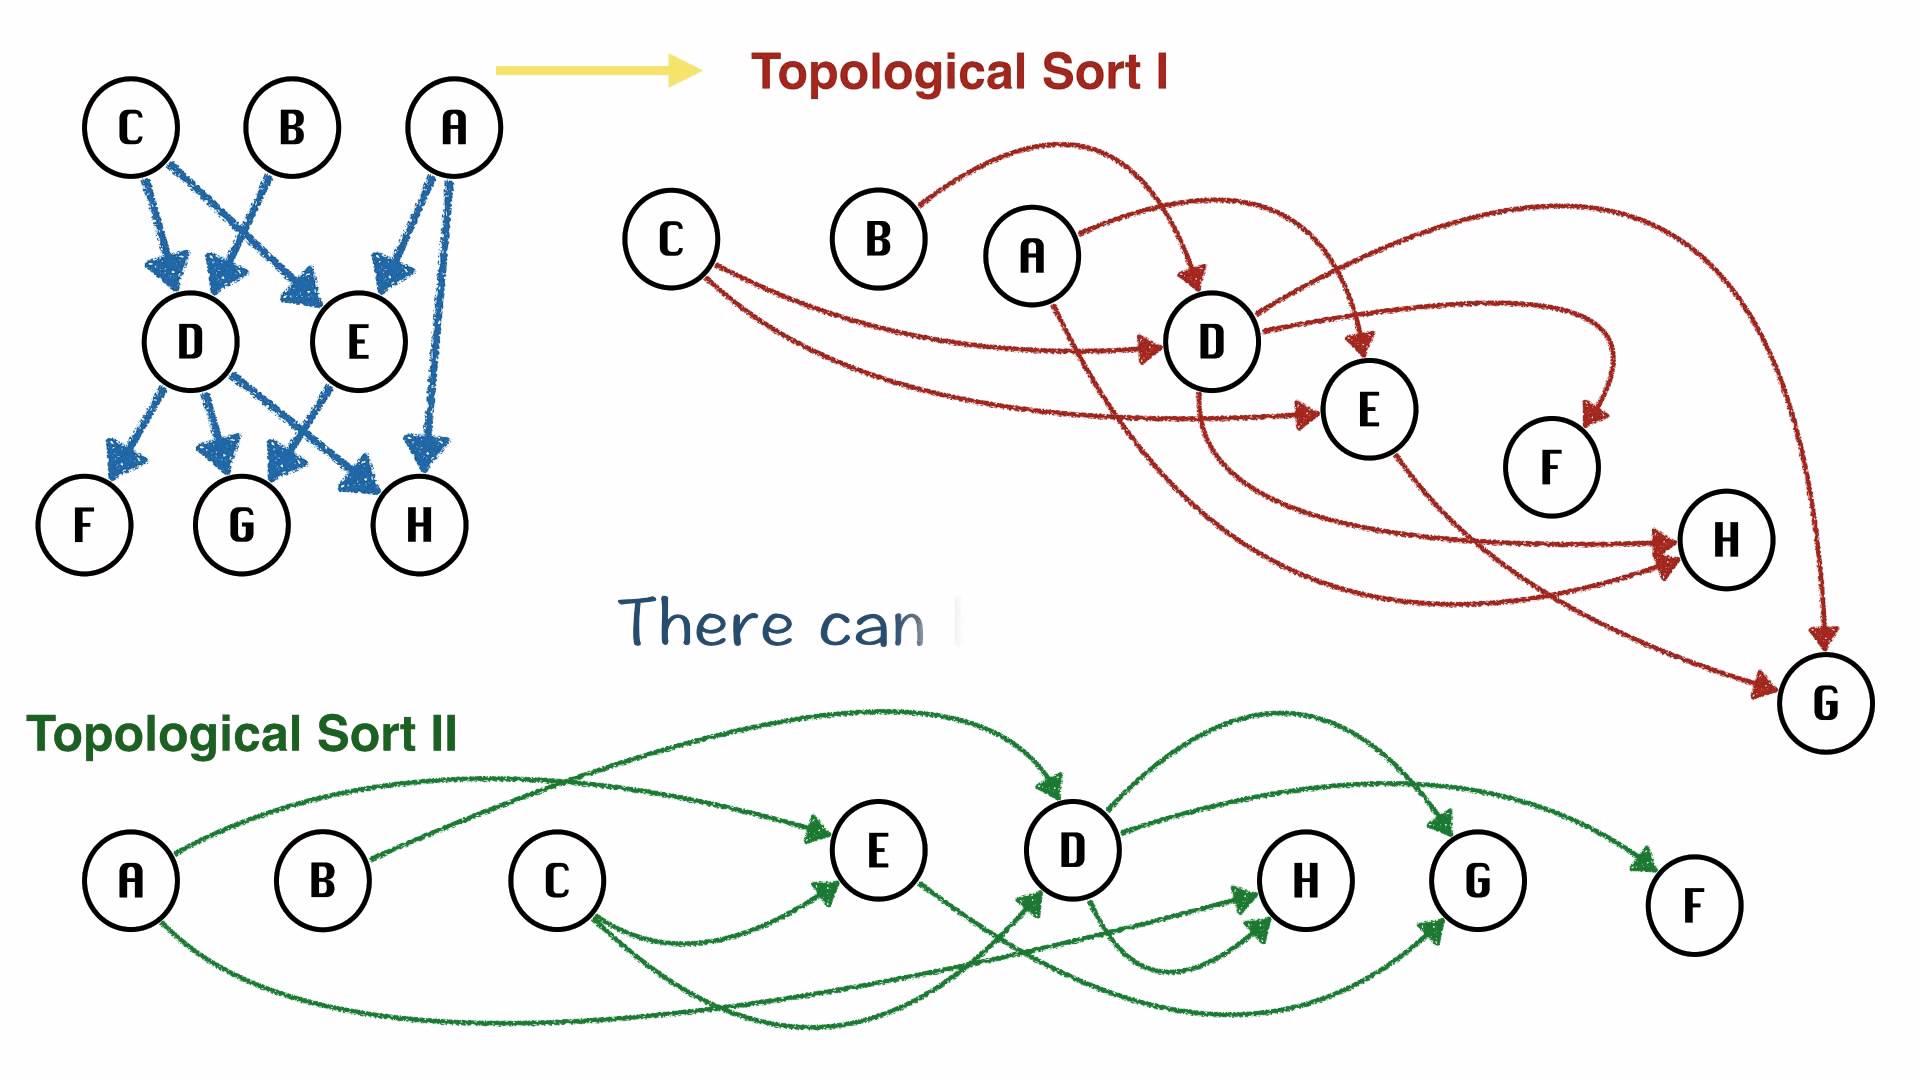
\includegraphics[width=\textwidth]{../images/DAGsort}
	\caption{DAG topological sorting}
	\end{figure}


Problem here is to find the shortest (largest works fine as well) between a two nodes $s$ called source and $d$ destination.
Consider, the DAG in figure \ref{fig:dagexample} with $s=A$ and $d=E$
	\begin{figure}
	\label{fig:dagexample}
	\centering
	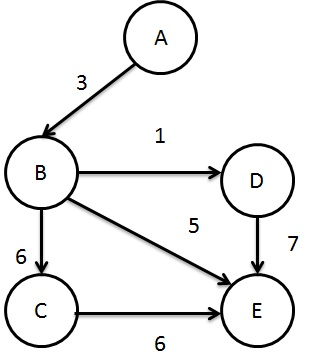
\includegraphics[width=0.5\textwidth]{../images/dagexample}
	\caption{DAG topological sorting}
	\end{figure}
In order to compute the shotest path it is usefult to think as follows. We know that any possible path that leads to $E$ eventually has to go through ieither $C,B,D$ cause those are the only edges that point inwards to $E$, out destination.
Is like willing to go to Rome which has three roads only  from outside the city to the center.
The length of the shortest path is clearly the following:
\[
	dist(A,E) = min\{dist(A,D)+weigth(D,E), dist(A,C)+weigth(C,E), dist(A,B)+weigth(B,E)\}
\]
As one can see from the above expression this formulation is made up of 3 smaller subproblems which can be solved the same way as the bigger problem.
One can ask the question, how much does the shortest path between $A$ and $D$ weights? Well it is formulaed the same way (ansering the question, how many inward edges $D$ has?):
\[
dist(A,D) = min\{dist(A,B) + weight(B,D)\} = dist(A,B) + weight(B,D)
\]
The nice thing about this approach is that if we work our way from A to E in a left to right manner (assuming DAG topological order) at time of computing any \textit{dist} subproblem we already have computed all relevant subproblems that allow us to solve the particular istance at hand (proceeding this way until we have solved all the subproblems).
A simple schematization of this ideas lead us to the pseudocode in listing (\ref{alg:dagshortest})
\begin{algorithm}\label{alg:dagshortest}
\Fn{DAG\_SHORTEST (A,E)}{
	\For{$i \gets 1$ \textbf{to} $n$} {
		$dist(A,n) \gets \infty$;
	}
	$dist(A,A) \gets 0$;\\
	\For{$v \in V \setminus\{A\}$ \texttt{in linearized order} }{
		$dist(A,v) \gets \min_{(u,v) \in E}{dist(A,u) + weight(u,v)}$
	}
}
\caption{DAG shortest path algorithm}
\end{algorithm}
Start at the very right. Distance from source to source is obviously zero, you don't need to move at all. 
Next node taken in consideration is (because they are linearly ordered) is $B$ for which the only edge having it as second node is $(A,B)$. Shortest path to 
$B$ is then $dista(A,A)=0 + weight(A,B) =3$ which totals $3$. Next ones is $C$ which has only one edge leading into it, $(B,C)$. $dist(A,C) = dist(A,B) + weight(B,C) = 3+6=9$.
Next one is $D$, again only one edge leading into it, $(B,D)$ which allows us to compute its shortest path from A: $dist(A,D) = dist(A,B) + weight(B,D) = 3 +1 =4$.
Next one is $E$ our destination node which has the following inwards edges $\{(D,E),(B,E), (C,E)\}$.Shortest path from $a$ to $E$ is then 
the minimum among the following quantities:
\[
	dist(A,B) + weight(B,E) = 3+5=8
\]
\[
	dist(A,C) + weight(C,E) = 7 + 9 = 16
\]
\[
	dist(A,D) + weight(D,E) = 2 +7 =9
\]
Minimum among $5,13,9$ is $5$ which happens to be the shortest path weight between $A$ and $E$ in graph in figure \ref{fig:dagexample}.
Is important to note here that we haven't find the actual \textit{path} but rather the weith of one of the possible shortest path! In order to find the shortest path we need to do some more work and record at each step i.e. at each subproblem solved or in other words when we find an intermediate shortest path value which is the parent node for which happen that the distance is minimal (Among all the inwards edges which one leads to the minimum weight?).
We will record all this informations in an associative array, \textit{parent}:
In the previous example when solving $dist(A,B)$ we found out that the shortest path was hopping through node $A$:  parent[B] = A;
For node $C$ shortest path was going through node B so parent[C] =B;
For node $D$ shortest path was going through node B so parent[D] =B;
For node $B$ shortest path was going through node B so parent[E] =B;
We can work the path backwards from the destination node and reconstruct all the hops using the \textit{parent} relationship.
$path(A,E) = E \rightarrow parent(E) \rightarrow  parent[parent[E]] \rightarrow  \ldots \rightarrow $ until we reach the souce node.

\section{Longest Increasing Subsequence}
The longest increasing subsequence is the problem of finding a subset $V_a=v_{a_1} \leq v_{a_2} \leq\ldots \leq v_{a_k}$, $a_1 < a_2 < \ldots < a_k$ and not other subsequence $V_b=v_{b_1}\leq v_{b_2}\leq \ldots \leq v_{b_l}$, $b_1 < b_2 < \ldots < b_l$ s.t. l > k.

The solution to this problems has to be a sequence of any size of element of the original collection s.t. the its overlall sum is \textbf{maximal}.

The naive approach leads to a $\Theta(2^n)$ algorithm which considers possible subset. Since there are an exponential number of such subsets this leads to a \textbf{exponential algorithm}.
We can do much better using DP.
Our goal is to recursively formulate the solution in terms of smaller problems than have no dependencies at all with the bigger ones.  Using the DAG analogy this means that for each subproblem to be solved the only information needed are solution to even smaller subproblems.

Let's work our way from the end of the array. What we know for sure is that the last element of the array can't be itself the first of a subsequence longer than one.
What we know about the second last element?
If a subsequence starts at this location then its lenght may be one or two depending weather this element is greater or less then the last one.
What about the third last? Again any subsequence starting at this location may be of lengths $1,2,3$ depeding weather it is greater than both the subsequent ones or only of one of them (no matter which one) or lesser than both.
This lead us to the following statement. Working our way backwards, at each location $i$ the longest subsequence starting at $i$ is the longest subsequence starting at any index greater than $i$ s.t. $V[j] > V[i]$ , $j>i$ i.e. the next element must be greater than the element at index $i$ (after all we are trying to find an increasing subsequence). 
Generalizing this idea we can formulate the solution as follows:
\[
LS(n) = 1+ \underset{ \underset{ V[i] > V[n]}{i > n} }{\max}{ LS[i]}
\]
 
In order to solve this problems we have created a list of subproblems with the following properties:
Problems are orderable and there exists a dependence between bigger and smaller problems. Bigger problems depends only on smaller problems, smaller problems depends on even smaller problems and so on until we reach the base case for which we already know the answer or we can compute it withoth using any other subproblem at all.
Each subproblem requires is dependent not only on one (smaller) subproblem but on all the smaller subproblems (the max operator iterate all subproblems till the base case)!
The complexity of solving one subproblem is then the complexity of finding the maximum value in a collection of values which can be done in $O(n)$. since we have to solve $n$ of this subproblems the complexity is quadratic $O(n^2)$. It is important to note that the max operator takes linear time \textbf{only} is we remember the solution to the smaller problems without recomputing them all the times they are required to be solved. This \textit{remembrance} is called \textbf{memoization} and is a key concept in \textbf{dymanic programming}. \textbf{Solution to problems that are required to be solved over and over have to be memoized}. 
Problems that exposes this pattern of decomposition i.e. that requires subproblems to be solved over and over again are said to have the property of \textbf{overlapping subproblems}. Memoization skyrocket the algorithm when a problem has this property.
The following is the pseudocode for the \textit{longest increasing subsequence}.


